\chapter{Literature Review}\label{ch:review}

\section{Brief Background}
The pricing of carbon emissions is a policy tool where emitters must pay
for carbon usage - thereby disincentivising reliance of unclean source of
energy. The conventional wisdom held by economists is a price on carbon
will provide an incentive for emitters to be `priced' out of using
unclean energy and choose to invest in clean renewable energy like
solar and wind. The economic theory behind carbon pricing is
simple - according to neoclassical economics markets are prone to
failure due to free riding. In the case of carbon, emitters free ride
by releasing carbon without considering the cost of carbon to the
planet and society. To remove the deadweight loss due to free riders, economists
propose placing a price on carbon to properly adjust emitting markets
to a socially optimal equilibrium price.

Presently, the great majority of humankind's emissions are not placed under
a price, with only 20\% of global emissions under a pricing
scheme~\cite{EconE}. Globally, the largest emissions trading schemes (ETS) are
run by the European Union (EU) and China. The EU ETS has recently been expanded
to cover around half of all emissions produced inside the EU (see
Figure~\ref{fig:ets}). Notable
economists suggest that for a carbon price to be effective in fulfilling the
Paris pledge then prices must stay between the range of \$40-80 per
tonne~\cite{EconE}.
As of 2020, the existing median price per tonne of carbon emissions is
only \$15~\cite{EconE}.

\begin{figure}[ht]
    \centering
    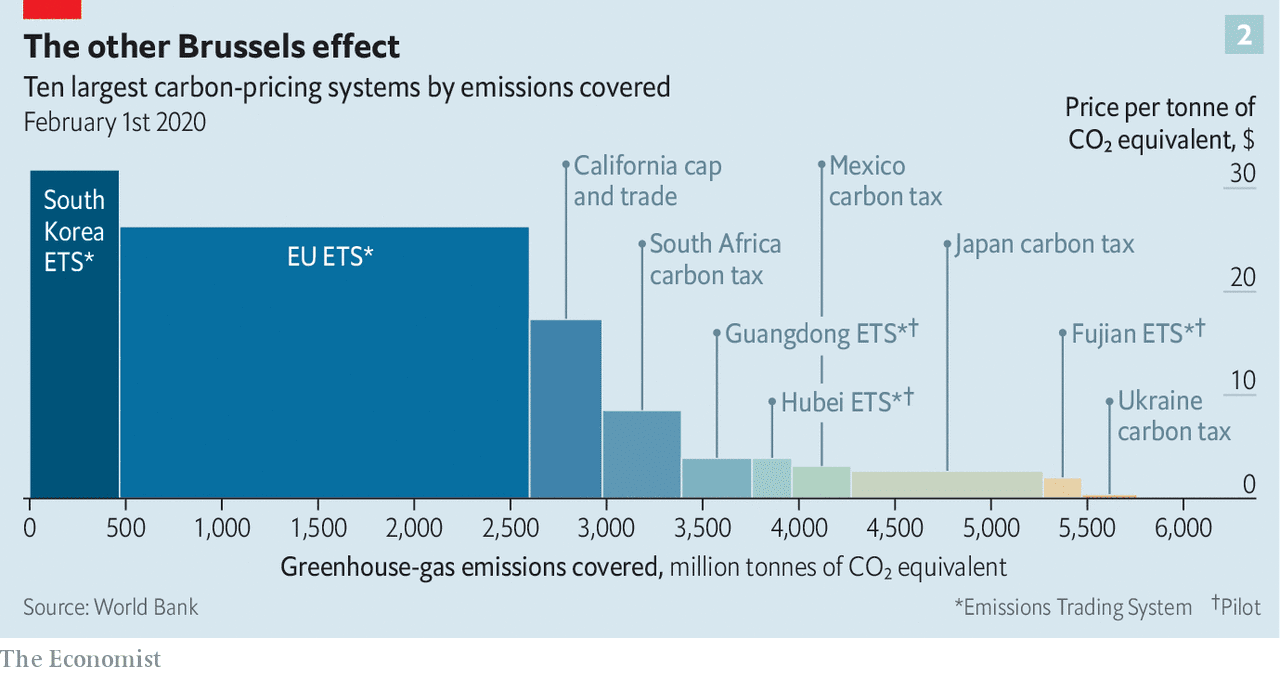
\includegraphics[scale=0.2]{photos/ets.png}
    \caption{Largest Emissions Trading Schemes}
    \label{fig:ets}
\end{figure}

Carbon prices are open to government manipulation from centralised
authorities and are often the subject of heated debates. An example
was the `axe the tax' campaign resulting in the abolishment of
the Australian ETS in 2014~\cite{EconE}. Moreoever, there is often
debate over where the money associated with carbon prices will go
- particularly in the case where an auction for carbon credits occurs.
If money raised from an ETS is used to lower taxes elsewhere in the economy then
opponents on the left of politics accuse the policy of not actively
fighting climate change. Generally, opponents on the right accuse carbon
prices of stifling economic growth - an example of an unecessary
government overreach.

The blockchain, which acts as an immutable ledger, has the potential to
deliver `trust' into the market for carbon. As opposed to being run
by a centralised authority like the government, it can instead be run
openly on the blockchain visible to all participants in the market for
carbon. Therefore, the openness of a blockchain ETS can be used to combat
its most fierce criticsm - which is its usage as a political tool.
A blockchain ETS can be designed so a `fee-and-dividend' is used, meaning
the distribution of payments can go straight back to the people thereby
incentivising long-term adoption~\cite{EconE}.

I will use the rapidly growing Hydrogen energy market - with its novel Hydrogen
certification process - to show how producers can pay for accrued
negative externalities. Hydrogen certificates can be automatically
submitted with a level of recorded emissions, whereby tokens are deducted
from a producer's carbon account upon submission. Smart contracts
(programs on the blockchain) will be used to represent the logic
of an ETS targetting hydrogen energy producers.

\section{Hydrogen Certificates}
The hydrogen market is a growing form of energy production created
from resources such as natural gas, coal, solar and wind. Hydrogen is
deemed a `clean fuel' because when it is consumed in a fuel cell
only water is produced. The hydrogen market is particularly important
for Australia since the industry is expected to create up to 7,600 jobs
and contribute \$11 billion a year to GDP~\cite{coag}. As part of an
effort to reduce cumbersome regulation associated with Hydrogen
markets internationl standards have been developed. Moreoever,
standards embedded into a \textit{hydrogen certificate} can
assist to manage the lifecycle of hydrodgen and ensure carbon
is not being emitted. As of 2020, there are eight international
hydrogen standards (see Table~\ref{tab:standards})
defining features such as safety and quality~\cite{stan}.

\begin{table}[ht]
    \centering
    \begin{tabular}{|l|l|}
        \hline
        \multicolumn{1}{|c|}{\textbf{Standard}} & \multicolumn{1}{c|}{\textbf{Description}}            \\ \hline
        AS 16110.1:2020                         & Safety                                               \\ \hline
        AS ISO 16110.2:2020                     & Performance                                          \\ \hline
        AS ISO 14687:2020                       & Fuel Quality                                         \\ \hline
        AS 22734:2020                           & Industrial, commercial, and residential applications \\ \hline
        SA TS 19883:2020                        & Safety of pressure swing adsorption systems          \\ \hline
        AS ISO 16111:2020                       & Transportation                                       \\ \hline
        AS ISO 19881:2020                       & Gaseous hydrogen                                     \\ \hline
        AS 19880.3:2020                         & Gaseous hydrogen – Fuelling stations                 \\ \hline
    \end{tabular}
    \caption{International Hydrogen Standards}
    \label{tab:standards}
\end{table}

To help develop standards, centralised certification authorities
are being developed to act as certification schemes for hydrogen.
One of the most popular such schemes is CertifHy - a European
scheme for hydrogen certification~\cite{certifhy}. Centralised
certification schemes provide services such as the issuance of
hydrogen certificates along with the ability for users to create
an account to track the registry of owned certificates. Generally,
hydrogen certificates have the ability to detail technical information
along with crucial greenhouse gas information.

A key problem with the centralisation of certification authorities is the
lack of openness involved. Customers become reliant on a key provider to
conduct certification, fostering less `trust' in the market for hydrogen.
Due to a lack of trust, a blockchain-based approach to hydrogen
certification would allow for greater extensibility in the different
certificates available. Crucially, an ETS with on-chain energy
certification can enforce carbon prices in a market. For example,
if a hydrogen certificate has not paid for its carbon usage using
the on-chain ETS - then due to the immutability and openness of the
blockchain such a certificate could be marked as not valid for
trading inside a commodity-market. This thesis will make the
assumption that such a rigorous certification scheme exists, and will
outline the technical details of a carbon market using energy certification
to place a price on carbon.

\section{Academic Blockchain Emission Trading Schemes}
\subsection{Bitcoin-based ETS}
An early adoption of blockchain carbon pricing was the
creation of a bitcoin-based emissions trading infrastructure model
in 2015~\cite{vic15}. The model proposed a blockchain called
Decentralised Carbon Emissions Trading Infrastructure (D-CETI)
inheriting a significant amount of the innovations created with
Bitcoin by Satoshi Nakamoto in 2009. The authors proposed that
the significant barriers limiting the effectiveness of the
major ETS schemes (EU ETS) was the lack of security and privacy
participants face in cardbon trading~\cite{vic15}. As a solution,
Bitcoin's at the time novel approach to security using hashed
transactions and computationally difficult hash puzzles was deemed by the
authors as an appropriate solution to the shortcomings of
the large ETS schemes.


\begin{figure}[ht]
    \centering
    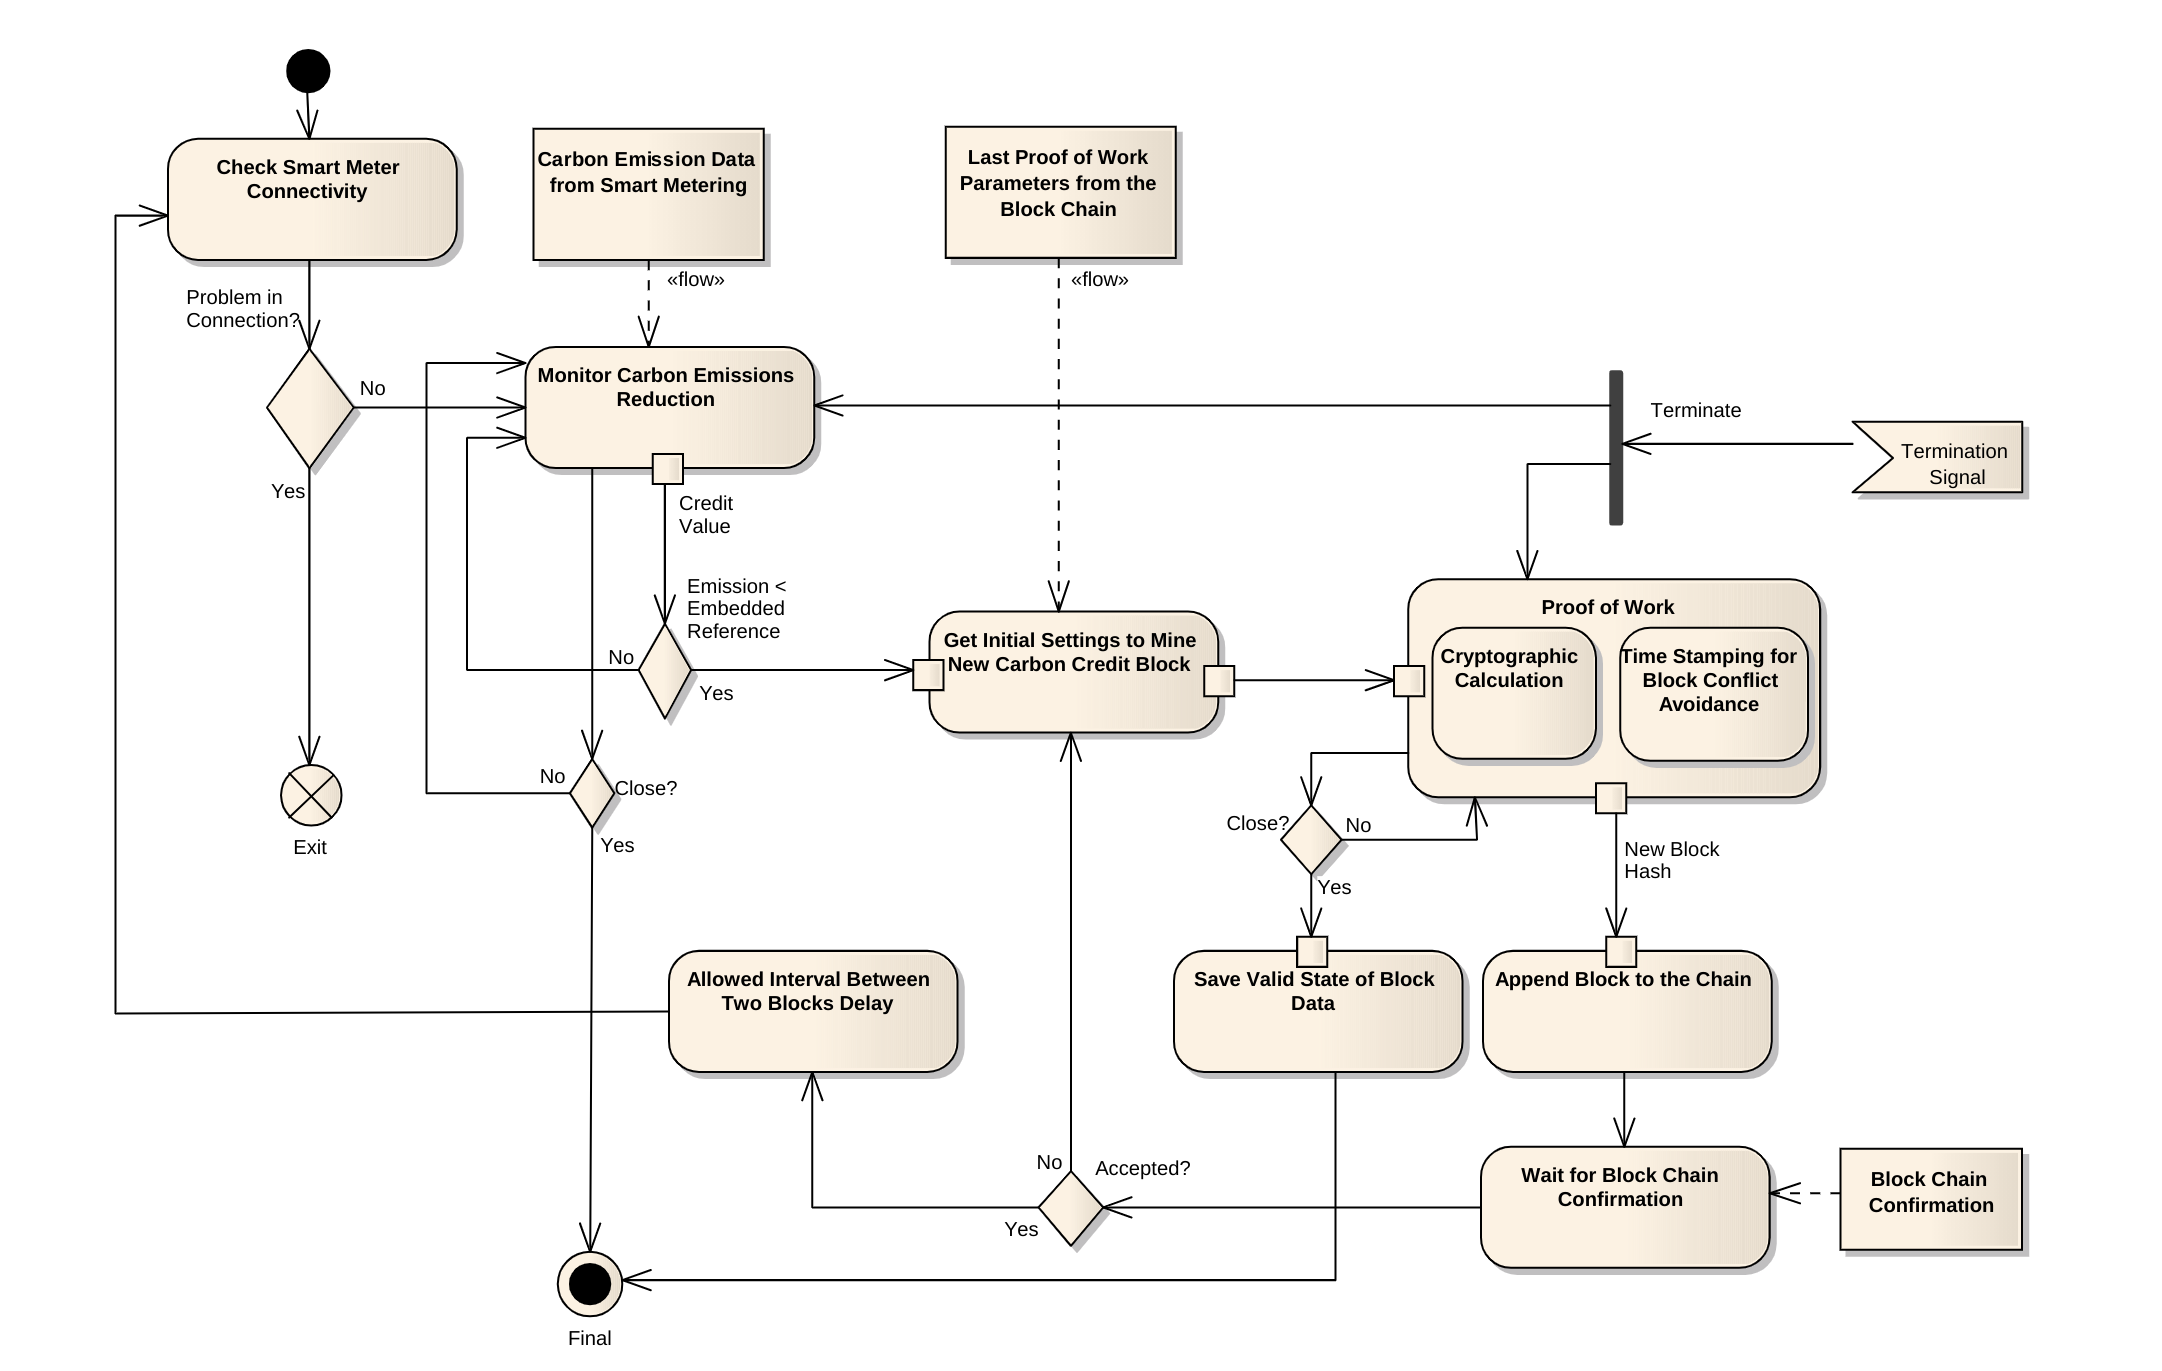
\includegraphics[scale=0.38]{photos/bitcoin.png}
    \caption{Bitcoin-based ETS}
    \label{fig:btc}
\end{figure}

In principal, the bitcoin-based ETS proposed functionality for
users to generate carbon tokens, register, sell,
and bid for credits. As a result, the system for a carbon market
was almost identical to the cryptocurrency Bitcoin with the
primary difference being the use of an ETS focused coin.
To deal with the throughput demands for an active ETS market,
the block generation rate on the chain became one block
every 150 seconds in contrast to Bitcoin's one block every
600 seconds~\cite{vic15}. Moreoever, participants in the bitcoin ETS market
would have to generate new blocks through miners solving cryptographic hash
puzzles (see Figure~\ref{fig:btc}).

The downsides to the bitcoin-based ETS are significant - the
throughput of the system is too low to ever be usable in an active
ETS market. Although increasing the throughput from 7 transactions
per second (TPS) for Bitcoin to roughly 28 TPS, such a solution
still relies on computationally expensive mining to achieve
system consensus~\cite{vic15}. Moreoever, Bitcoin's reliance on
hash puzzles requires the continuous consumption of carbon emitting
energy - potentially worsening the market failure which the ETS is aiming to
remedy.

The bictoin-based ETS relies on a primitive form of smart contracts
inherited from \textit{Bitcoin Script} - meaning the smart contracts
are not turing complete. Therefore, it would not be possible to
express detailed business logic such as the auctioning of tokens
or custom carbon prices into such an architecture. Simply stated -
a Bitcoin-based ETS is insufficient for a carbon market.

\subsection{Blockchain-based Smart Grid}
A more innovative public blockchain, such as Ethereum, has been
proposed as a system to host local energy markets~\cite{beer}.
The benefit of using Ehtereum primarily comes from the use of
a turing-complete Ethereum Virtual Machine allowing for
the creation of complex smart contracts. Hence, the creation
of an intricate local energy market becomes possible through a
distributed programs written in a high level language (such as Solidity) which is then compiled into Etherum bytecode. The
researchers found the use of Ethereum as a local energy market
allowed for electricy cost reductions across a
model scenario~\cite{beer}.

Despite the technical feasibility of developing an ETS on
Ethereum, the platform is not suitable due to technical limitations.
The researchers acknowledged that further analysis into the
suitability of public blockchains for energy markets is
required~\cite{beer}. Specifically, Ethereum supports a 25 TPS for
system throughput~\cite{racz}.
For an active ETS in an emerging industry such
as hydrogen production, such a low system throughput would do
damage to the usability and customer satisfaction involved in
carbon trading. Moreover, Ethereum is being actively developed
and has planned forks due to a move towards a proof of stake
consensus algorithm~\cite{pos} - making it unstable
for a certificate-based ETS requiring customer trust.

\subsection{Reputation-based ETS Blockhain}

Researchers in 2017 proposed the use of a reputation-based
ETS with a blockchain infrastructure,
employing a permissioned blockchain to overcome
the throughput issues asscoiated with public
blockchain networks~\cite{KHAQQI20188}. The researchers concluded
that the environment \textit{Multichain} would be a good
candidate for a blockchain ETS due to its support for
a system throughput with up to 1000 theoretical TPS~\cite{KHAQQI20188}. Similar to
previous blockchain carbon markets, the researchers made smart
meters and the trading of tokens
central components to the functioning of
the system - as observed in Figure~\ref{fig:rep}.

\begin{figure}[ht]
    \centering
    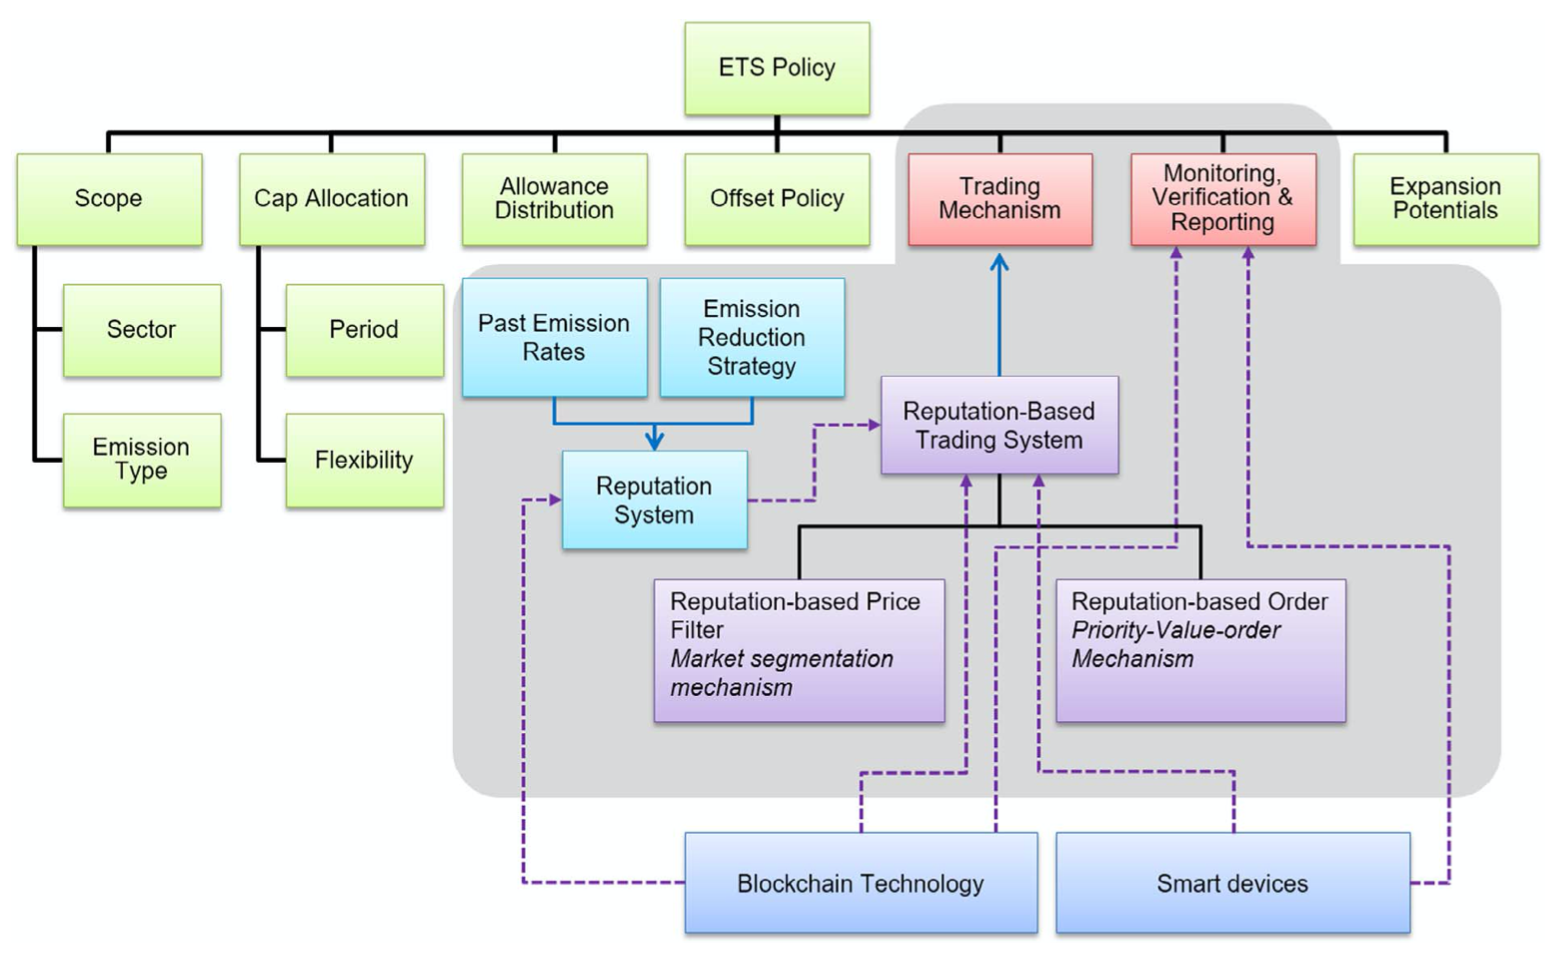
\includegraphics[scale=0.37]{photos/reputation.png}
    \caption{Reputation-based Blockchain ETS}
    \label{fig:rep}
\end{figure}

Khaqqi et al believed that the critical element holding back
the success of a blockchain ETS is the lack of a reputation
model present in the pricing of carbon tokens. Often,
markets can increase in quality, and grow when there is a way
to remove systemic information asymmetry~\cite{KHAQQI20188}
(as an example consider online marketplaces and seller scores).
Therefore, Khaqqi et al proposed the incorporation of the
`carbon reputation' of a seller into the pricing of carbon tokens.
As observerd in Equation~\ref{eqn:pv}, changing the `reputation'
parameter to factor a seller's carbon emissions can influence the price
offered to agents buying tokens in the
ETS blockchain~\cite{KHAQQI20188}.

\begin{equation}
    \text{PV} =
    \frac{\text{askingprice}}
    {\text{reputation} - \text{basedfactor}}
    \label{eqn:pv}
\end{equation}

Despite offering a solution with more
system throughput than both Ethereum and Bitcoin-based offerings
there has not been a general movement towards
a carbon market with reputation pricing. A weakness of the
architecture employed by Khaqqi et al is the requirement that
prices must automatically reflect the `carbon reputation' of
sellers in the marketplace. Forcing reputation systems
upon users is disrespecting of user freedom, and
should be made an option and not a requirement for
participating in the system. Moreover, as The Economist
stated: public criticism and politics are key factors holding
back the success of a carbon market~\cite{EconE}.
The simplicity of energy certification could be
combined with \textit{optional} reputation pricing to deliver satisfaction
amongst producers.

\subsection{Hyperledger Carbon Market}
In 2018 Yuan et al developed a carbon market using the
permissioned blockchain network Hyperledger Fabric~\cite{article}.
The researchers identified that a core issue holding back the
success of existing ETS systems was a lack of trust
along with data security problems associated with centralised carbon
markets.
The researchers determined the Hyperledger project as offering
a customisable ledger structure well suited to the security
needs of a distributed carbon market. As such, a simple
architecture comprising of nodes offering an environmental
agency, permit approver, traders and a trading centre was designed. The
`approver' in the Hyperledger ETS system manually inspects
projects and allocates permits to allow for access to a `trading
centre' (as seen in Figure~\ref{fig:htrad}).

\begin{figure}[ht]
    \centering
    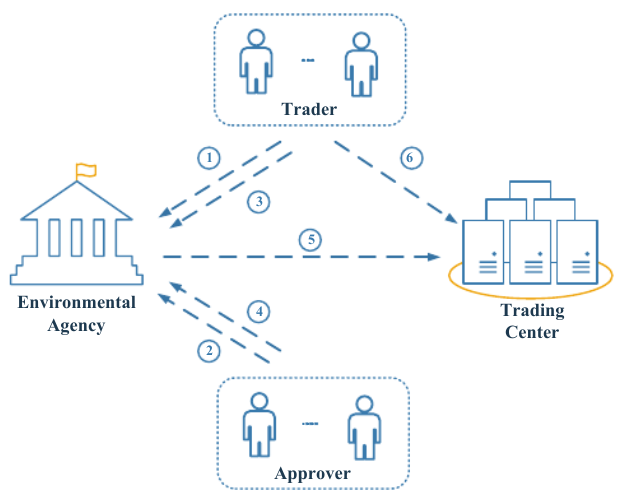
\includegraphics[scale=0.6]{photos/hyptrade.png}
    \caption{Hyperledger Carbon Market}
    \label{fig:htrad}
\end{figure}

The algorithms employed in trading carbon permits are
trivial by design - the trading mechanism employs a smart contract
checking the number of permits in the seller's account. If the
seller has a valid number of permits, then the trade is executed
and carbon permits are allowed to be traded between market
participants~\cite{article}. The architecture employs a single
Hyperledger \textit{channel} allowing for the ordering of transactions
between both the environmental agency and the trading centre.
Interaction with the blockchain happens through a HTTP server
offering RESTful APIs. Within the Hyperledger blockchain there
are two smart contracts: an application contract (AC) for the
environmental agency and a trading contract (TC) for emissions
trading~\cite{article}.

The Hyperledger carbon market's innvoation comes from
using the new technology of Hyperledger - which offers
superior TPS performance and architectural modularity. Yuan et al
were able to get the Hyperledger carbon market to handle
up to 340 requests per second~\cite{article} - significantly
more than what the Ethereum blockchain offers. Despite the
success coming from Hyperledger adoption the proposed system is
trivial and requires significant manual approval on the
behalf of a centralised environment agency. A better
approach would make use of an existing form of automation (such
as certification) to spend permits. Moreoever, making smart contracts
more complex through \textit{optional} carbon reputations
would improve the quality of the market for carbon~\cite{KHAQQI20188}.

\section{Enterprise Energy Markets}

\subsection{PowerLedger}

PowerLedger is a private energy company based in Australia
who launched a blockchain microgrid in 2016. The company is
Australia's first peer-to-peer energy trading network~\cite{power}. PowerLedger allows for access to the
energy market using a \textit{POWR} token, which provides
electrical units (in kWh) and market pricing
mechanisms. \textit{POWR} tokens are subsequently
escrowed for a \textit{Spark} token to access the
PowerLedger ecosystem. PowerLedger provides a public
blockchain layer built using Ethereum for
coin markets which links to PowerLedger's private
permissioned blockchain~\cite{power}.

PowerLedger offers a pragmatic solution to energy markets.
PowerLedger highlights how trust can be delivered to
an energy market hosting a consortium of energy sources.
Although not driven by energy certification, PowerLedger
demonstrates the technical feasibility of
a blockchain for energy in a diverse and growing market.

\subsection{SOLShare}

SOLShare is a blockchain-based energy market
for Bangladesh. The blockchain offers an effective solution
due to the presence of over four million
rooftop panels and batteries powering the electricity grid of
Bangladesh~\cite{powersol}. The platform requires
a proprietary technology called a \textit{SOLBox} allowing for
a user to either sell or buy electricity. SOLShare
provides a motivating example of an energy
blockchain application delivering value and trust to
hundreds of customers~\cite{powersol}.

\section{Hyperledger}
The Hyperledger project is an open-source collection of tools and
frameworks that are created for developing permissioned blockchains.
A permissioned blockchain contrasts directly with popular
public blockchains such as Bitcoin and Ethereum: precisely
because agents on the blockchain are able to be identified.
The Hyperledger project follows a philosophy of modularity
and interoperability of the blockchain, meaning the
vision of Hyperledger is to have blockchains with a pluggable architecture
that can seamlessly communicate with another Hyperledger blockchain~\cite{hypa}.

\subsection{Hyperledger Fabric}
One of the most popular Hyperledger frameworks is Hyperledger Fabric:
a modular and extensible framework for developing blockchain
applications~\cite{And18}. The primary technological innvoation of
Fabric is the introduction of a novel `execute-order-validate' paradigm
for transactions. A `execute-order-validate' architecture means that
transactions with accompanying smart contracts are first
executed by peers on the network before being sent to a specified
ordering service, which broadcasts the transactions amongst the blockchain
network (as observed in Figure~\ref{fig:exe}).
The `execute-order' architecture directly contrast with
Ethereum's `order-execute' approach which requires \textit{active replication}
of transactions amongst all nodes in the system, thereby making consensus
difficult to achieve.

\begin{figure}[ht]
    \centering
    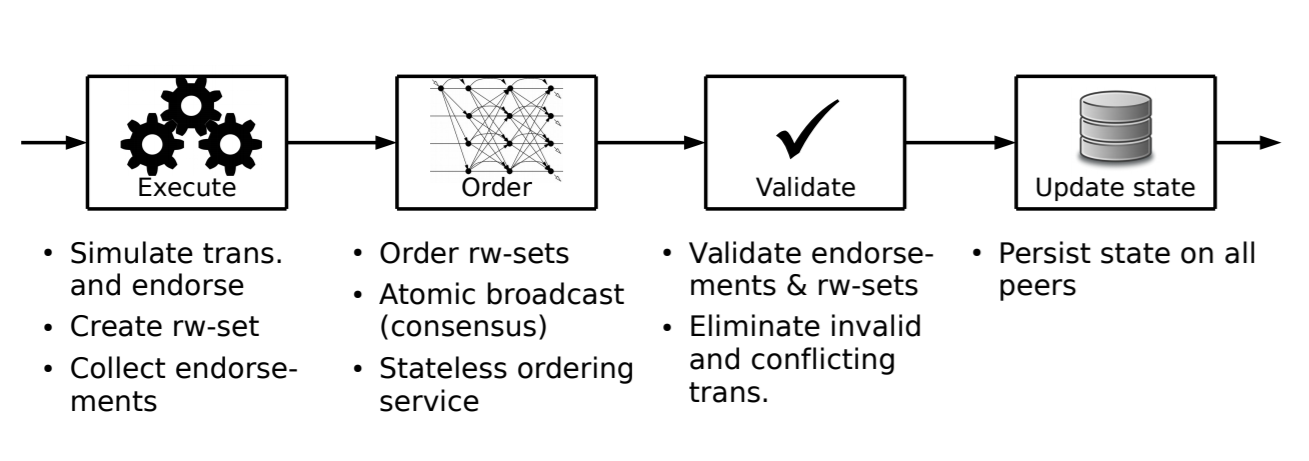
\includegraphics[scale=0.5]{photos/execute.png}
    \caption{Execute-order Architecture}
    \label{fig:exe}
\end{figure}

During the execution phase of Fabric a client creates a \textit{transaction
    proposal} to send to a collection of endorsers on a specific
\textit{channel}. The proposal contains an item called \textit{chaincode}
acting as a program running inside a secured Docker container which has
the ability to manage and manipulate the state of the ledger.
A client will collect endorsements from nodes until an
\textit{endoresement policy} has been satisfied, whereby the transaction
is then sent to the ordering service. The technological innovation
associated with the execution phase is the toleration of
non-determinism in transactions, meaning non-determinism only threatens the
life of a particular transaction and not consensus on the blockchain.
The execution phase of Fabric allows for a smart contracts in a
carbon market to be written
in a general programming language like Go or Javascript~\cite{And18}.

The ordering phase of Fabric established a `total ordering' of transactions
on a channel allowing for consensus in the system to be achieved~\cite{And18}.
Fabric has specific nodes labeled \textit{Ordering Service Nodes} (OSN)
whose purpose is to order transactions (and not engage in either
execution or validation of transactions). Along with the OSNs there
is an accompanying protocol called \textit{gossip} allowing for blocks
to be distributed efficiently amongst peers on the ledger
(see Figure~\ref{fig:harch}). Through the separation of ordering to
specific nodes, Fabric is able to make system consensus modular.
Hence, a popular consensus algorithm in Fabric is \textit{Raft}: a Crash Fault
Tolerant (CFT) consensus algorithm. The \textit{Raft} algorithm uses
a `leader follow' approach where a leader is elected per channel to
do the ordering of transactions~\cite{raft}. By using Fabric with
\textit{Raft} as a consensus algorithm a carbon market would be able
to replicate a theoretical TPS of up to 3420~\cite{And18}. Moreoever,
such a carbon market would be modular with a modifiable consenus
algorithm suiting the requirements of market participants.

\begin{figure}[ht]
    \centering
    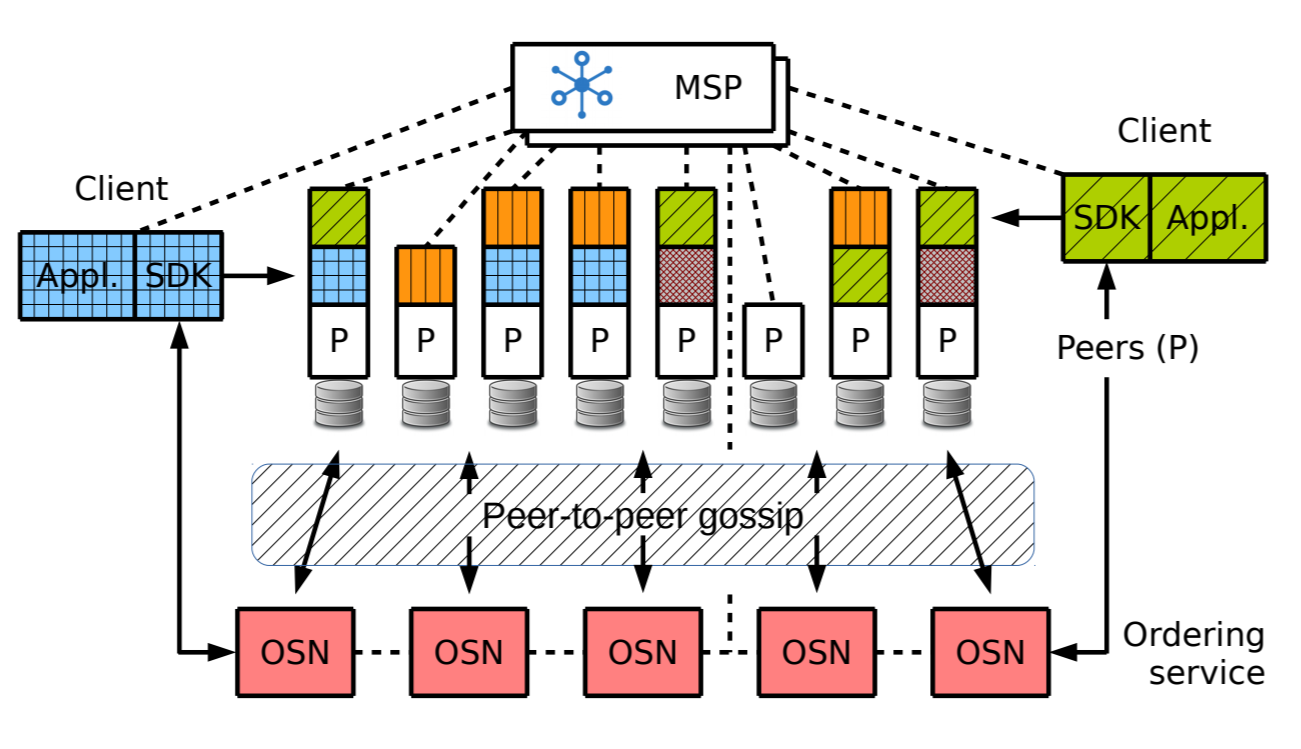
\includegraphics[scale=0.4]{photos/hyperarch.png}
    \caption{Hyperledger Architecture}
    \label{fig:harch}
\end{figure}

The final phase of Fabric is the validation phase whereby
\textit{validation system chaincode} is run by nodes to check the
validity of transactions~\cite{And18}. As part of the
validation phase a check is
performed to determine if the endorsement policy for transaction
chaincode is satisfied.
Due to the enterprise focus of Hyperledger, transactions that
are determined as \textit{invalid} are persisted to the ledger to allow
for easier auditing of transaction. The validation phase of Hyperledger
fosters trust in a carbon market by ensuring market fraud is persisted to the
blockchain and caught in subsequent audits on the state of the ledger.
Potential fraud in a carbon market would be persisted to the ledger
and caught on audits of the blockchain.

\section{Problem Statement}

The success of the long-term adoption of a blockchain-based carbon
market is reliant on the trust market patiticpants place into the
system. Previous blockchain carbon markets have been held back by
inefficient implementations with low system throughput - such as
the bitcoin-based emissions trading scheme~\cite{vic15}. Often, when
more innovative blockchain architectures are researched for carbon markets
they come coupled with features such as `reputation' pricing that
participants may want to opt-out of~\cite{KHAQQI20188}. Within the
literature for carbon markets, there is a need for a solution that is
both easy-to-use whilst also respecting of the freedom of participants.

I suggest a new approach to carbon markets with energy certificates.
Instead of relying on manual permit approvals, I suggest a novel approach
to carbon markets where producers of carbon can automatically consume
carbon tokens through the use of energy certificates. I will motivate
my certificate-driven carbon market with the use of on-chain
hydrogen certificates. Consuming carbon tokens will therefore become
a natural part of the lifecycle of a hydrogen certificate. Such a
carbon market has the objective of rapidly incentivising the use of
cleaner sources of hydrogen energy.

To encourage transparency in carbon markets, I will use the high throughput
blockchain Hyperledger Fabric. Hyperledger offers a permissioned
blockchain allowing for hydrogen producers to be identified when consuming
carbon tokens. Moreoever, I will provide the option for buyers of
carbon tokens to filter prices according to the carbon reputation of
sellers, thereby encouraging the ethical exchange of carbon tokens.

\section{Example Scenario}

A user will want to use the carbon market to `spend' hydrogen energy
certificates. A user will be able to observe on a dashboard all unspent
hydrogen energy certificates, and submit such certificates to the
carbon market to `spend carbon tokens'. A user will be allowed to
observe an open market for carbon tokens, and purchase or sell a quantity of
carbon tokens at a given price per token. The user will be given the
optional ability to filter open market carbon token offers by the
\textit{carbon reputation} of the seller - meaning the user can choose not
to observe token offers from carbon emitting hydrogen producers. A user
will be allowed to directly purchase carbon tokens from the carbon market
authority at a given price per token - typically at a price above what the
open market is offering.

\section{Aims and Outcomes}

This thesis aims to use on-chain hydrogen energy certificates to
outline how carbon markets can be efficiently run using a blockchain.
I propose an implementation of a carbon market using Hyperledger
Fabric, with the assumption that an already existing
certification scheme exists. Developed alongside the carbon
market blockchain will be a user interface to allow for the
exchange of carbon tokens between market participants.

The outcome of the thesis is a blockchain application with an architecture
performing the automatic spending of carbon tokens using hydrogen
energy certificates. The application is intended to be used by
producers of hydrogen energy who are seeking to buy and sell carbon
tokens to deal with an associated level of emissions resulting from
hydrogen production. The aim of the thesis is not
to solve the economic problem of developing an efficient
market for carbon - instead the technical feasibility of
a blockchain carbon market employing energy
certificates is explored.

The primary outcomes are listed below:
\begin{enumerate}
    \item Ability to purchase carbon tokens from other hydrogen producers.
    \item Ability to sell carbon tokens to other hydrogen producers.
    \item Ability to view hydrogen certificates requiring payment with
          carbon tokens.
    \item Ability to filter token sale offers based on the `carbon reputation'
          of a hydrogen producer.
    \item Creation of a user interface for a seller to interact with a carbon
          market.
\end{enumerate}